\documentclass{standalone}
\usepackage{tikz}
\usetikzlibrary{patterns, positioning}
\usepackage[sfdefault]{ClearSans} %% option 'sfdefault' activates Clear Sans as the default text font
\usepackage[T1]{fontenc}

\begin{document}
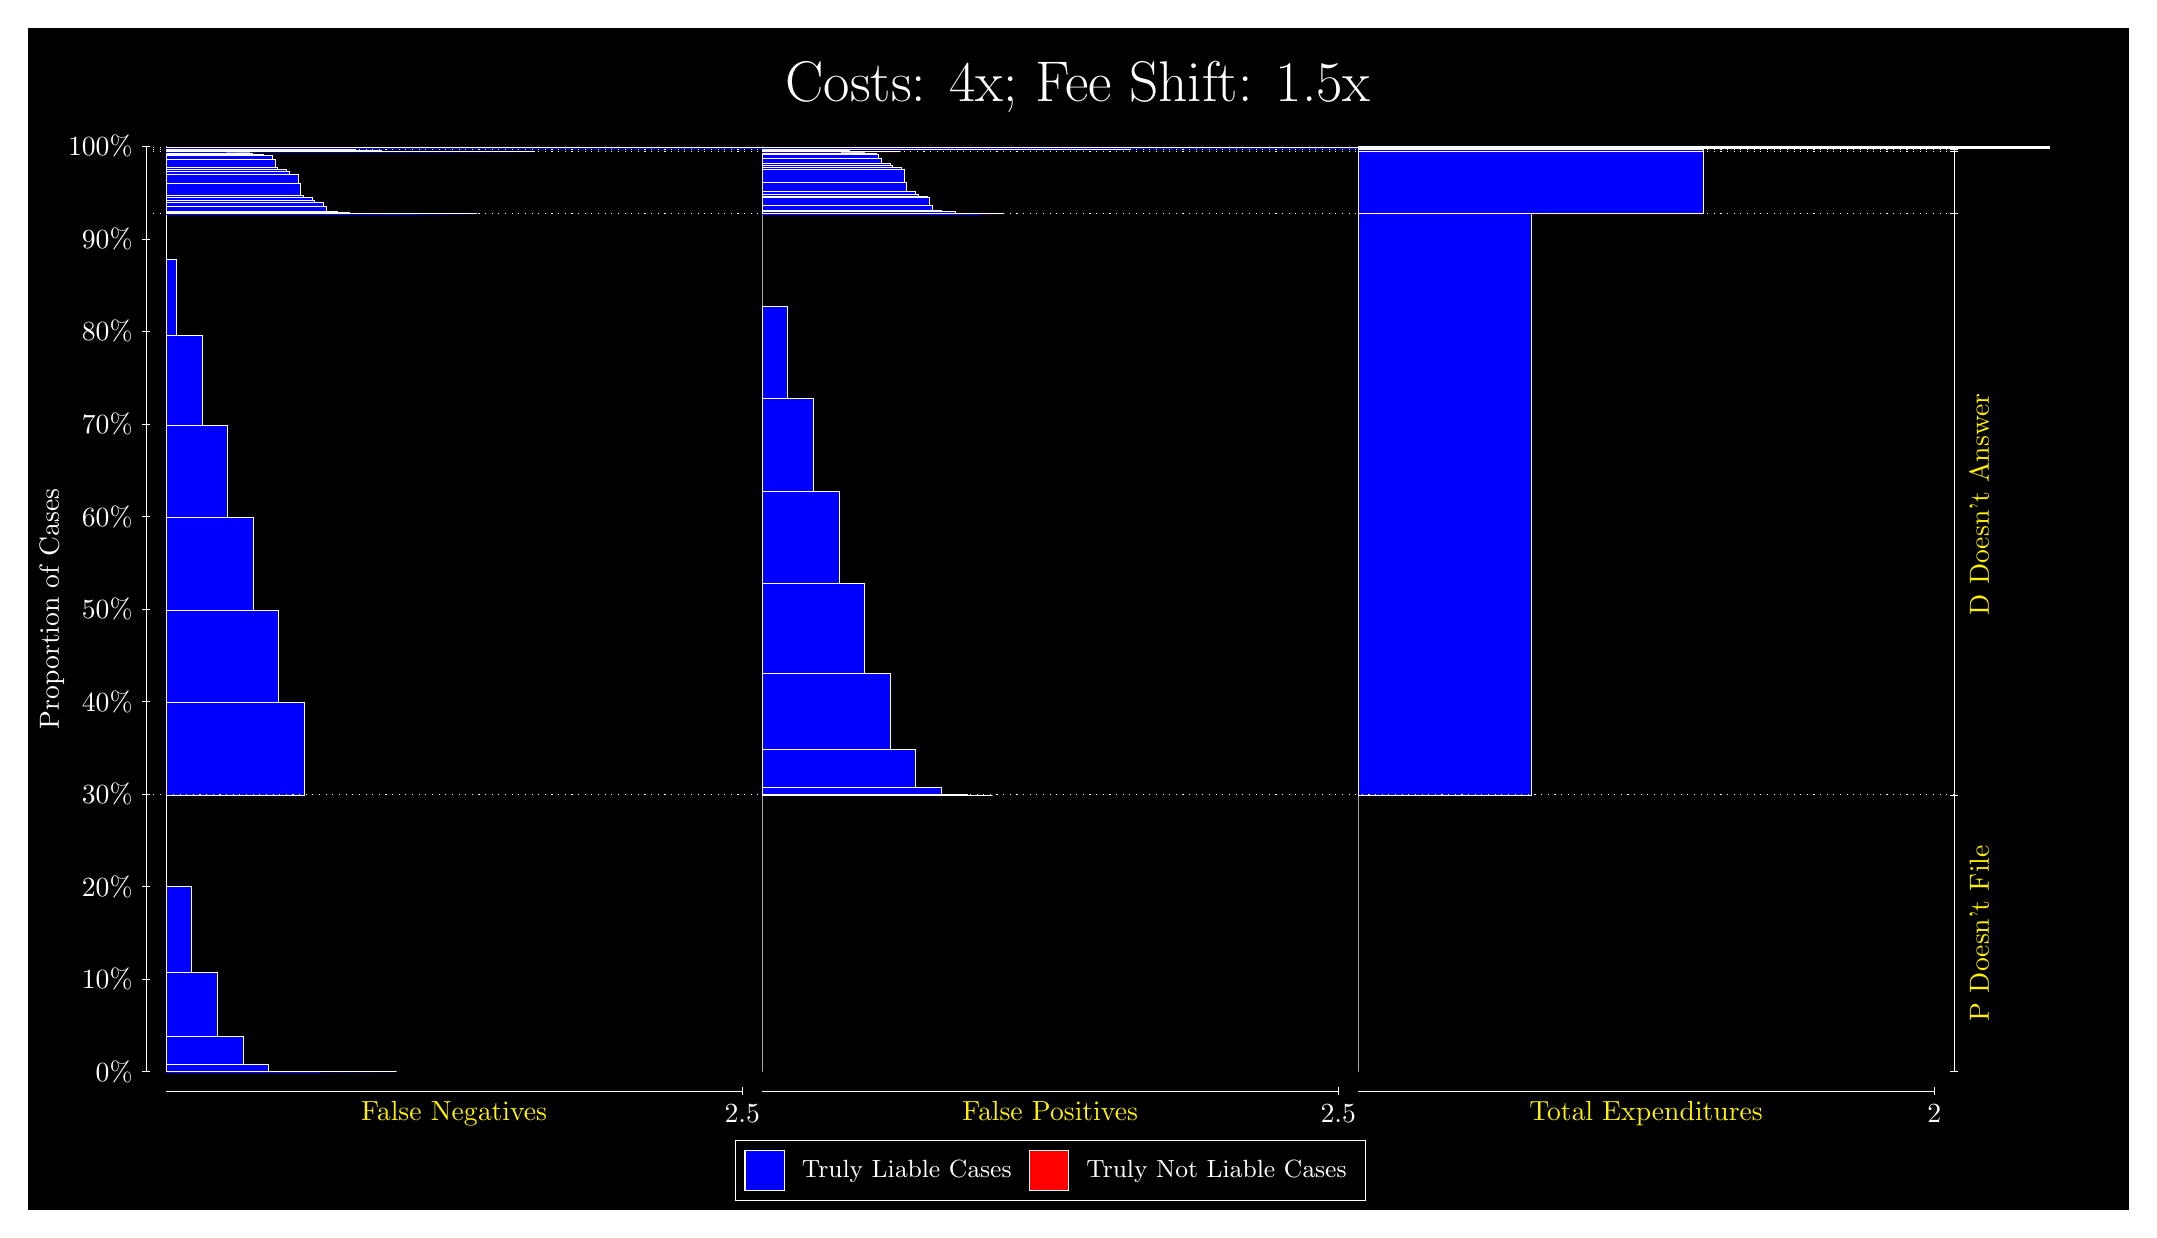
\begin{tikzpicture}
\draw[fill=black] (0,0) rectangle (26.667,15);
\draw[text=white] (0,13.5) rectangle (26.667,15) node[midway] {\huge Costs: 4x; Fee Shift: 1.5x};
\draw[white, very thin] (1.5,1.75) -- (1.5,13.5);
\node[rotate=90, text=white, anchor=center] at (0.3, 7.625) {Proportion of Cases};
\draw[white, very thin] (1.45,1.75) -- (1.55,1.75);
\node[text=white, anchor=east] at (1.45, 1.75) {0\%};
\draw[white, very thin] (1.45,2.925) -- (1.55,2.925);
\node[text=white, anchor=east] at (1.45, 2.925) {10\%};
\draw[white, very thin] (1.45,4.1) -- (1.55,4.1);
\node[text=white, anchor=east] at (1.45, 4.1) {20\%};
\draw[white, very thin] (1.45,5.275) -- (1.55,5.275);
\node[text=white, anchor=east] at (1.45, 5.275) {30\%};
\draw[white, very thin] (1.45,6.45) -- (1.55,6.45);
\node[text=white, anchor=east] at (1.45, 6.45) {40\%};
\draw[white, very thin] (1.45,7.625) -- (1.55,7.625);
\node[text=white, anchor=east] at (1.45, 7.625) {50\%};
\draw[white, very thin] (1.45,8.8) -- (1.55,8.8);
\node[text=white, anchor=east] at (1.45, 8.8) {60\%};
\draw[white, very thin] (1.45,9.975) -- (1.55,9.975);
\node[text=white, anchor=east] at (1.45, 9.975) {70\%};
\draw[white, very thin] (1.45,11.15) -- (1.55,11.15);
\node[text=white, anchor=east] at (1.45, 11.15) {80\%};
\draw[white, very thin] (1.45,12.325) -- (1.55,12.325);
\node[text=white, anchor=east] at (1.45, 12.325) {90\%};
\draw[white, very thin] (1.45,13.5) -- (1.55,13.5);
\node[text=white, anchor=east] at (1.45, 13.5) {100\%};

\draw[white, very thin] (24.457,1.75) -- (24.457,13.5);
\draw[white, very thin] (24.407,1.75) -- (24.507,1.75);
\node[anchor=west] at (24.407, 1.75) {};
\draw[white, very thin] (24.407,5.264) -- (24.507,5.264);
\node[anchor=west] at (24.407, 5.264) {};
\draw[white, very thin] (24.407,12.645) -- (24.507,12.645);
\node[anchor=west] at (24.407, 12.645) {};
\draw[white, very thin] (24.407,13.433) -- (24.507,13.433);
\node[anchor=west] at (24.407, 13.433) {};
\draw[white, very thin] (24.407,13.463) -- (24.507,13.463);
\node[anchor=west] at (24.407, 13.463) {};
\draw[white, very thin] (24.407,13.48) -- (24.507,13.48);
\node[anchor=west] at (24.407, 13.48) {};
\draw[white, very thin] (24.407,13.5) -- (24.507,13.5);
\node[anchor=west] at (24.407, 13.5) {};

\draw[white, very thin, fill=blue] (1.75,1.75) rectangle (4.6775,1.75);
\draw[white, very thin, fill=blue] (1.75,1.75) rectangle (4.3523,1.75);
\draw[white, very thin, fill=blue] (1.75,1.75) rectangle (4.027,1.75);
\draw[white, very thin, fill=blue] (1.75,1.75) rectangle (3.7017,1.7503);
\draw[white, very thin, fill=blue] (1.75,1.7503) rectangle (3.3764,1.7576);
\draw[white, very thin, fill=blue] (1.75,1.7576) rectangle (3.0511,1.8361);
\draw[white, very thin, fill=blue] (1.75,1.8361) rectangle (2.7258,2.1984);
\draw[white, very thin, fill=blue] (1.75,2.1984) rectangle (2.4006,3.0086);
\draw[white, very thin, fill=blue] (1.75,3.0086) rectangle (2.0753,4.0995);
\draw[white, very thin, fill=red] (1.75,4.0995) rectangle (1.75,4.0995);
\draw[white, very thin, fill=blue] (1.75,4.0995) rectangle (1.75,5.264);
\draw[white, very thin, fill=blue] (1.75,5.264) rectangle (3.5065,6.439);
\draw[white, very thin, fill=blue] (1.75,6.439) rectangle (3.1812,7.614);
\draw[white, very thin, fill=blue] (1.75,7.614) rectangle (2.856,8.7889);
\draw[white, very thin, fill=blue] (1.75,8.7889) rectangle (2.5307,9.9616);
\draw[white, very thin, fill=blue] (1.75,9.9616) rectangle (2.2054,11.105);
\draw[white, very thin, fill=blue] (1.75,11.105) rectangle (1.8801,12.063);
\draw[white, very thin, fill=red] (1.75,12.063) rectangle (1.75,12.063);
\draw[white, very thin, fill=blue] (1.75,12.063) rectangle (1.75,12.645);
\draw[white, very thin, fill=blue] (1.75,12.645) rectangle (5.7022,12.645);
\draw[white, very thin, fill=blue] (1.75,12.645) rectangle (5.5558,12.645);
\draw[white, very thin, fill=blue] (1.75,12.645) rectangle (5.4094,12.645);
\draw[white, very thin, fill=blue] (1.75,12.645) rectangle (5.3769,12.645);
\draw[white, very thin, fill=blue] (1.75,12.645) rectangle (5.2631,12.645);
\draw[white, very thin, fill=blue] (1.75,12.645) rectangle (5.2305,12.645);
\draw[white, very thin, fill=blue] (1.75,12.645) rectangle (5.1167,12.645);
\draw[white, very thin, fill=blue] (1.75,12.645) rectangle (5.0842,12.645);
\draw[white, very thin, fill=blue] (1.75,12.645) rectangle (5.0516,12.645);
\draw[white, very thin, fill=blue] (1.75,12.645) rectangle (4.9378,12.645);
\draw[white, very thin, fill=blue] (1.75,12.645) rectangle (4.9052,12.645);
\draw[white, very thin, fill=blue] (1.75,12.645) rectangle (4.7914,12.645);
\draw[white, very thin, fill=blue] (1.75,12.645) rectangle (4.7589,12.645);
\draw[white, very thin, fill=blue] (1.75,12.645) rectangle (4.7263,12.645);
\draw[white, very thin, fill=blue] (1.75,12.645) rectangle (4.6125,12.645);
\draw[white, very thin, fill=blue] (1.75,12.645) rectangle (4.58,12.645);
\draw[white, very thin, fill=blue] (1.75,12.645) rectangle (4.4661,12.645);
\draw[white, very thin, fill=blue] (1.75,12.645) rectangle (4.4336,12.645);
\draw[white, very thin, fill=blue] (1.75,12.645) rectangle (4.4011,12.645);
\draw[white, very thin, fill=blue] (1.75,12.645) rectangle (4.2872,12.645);
\draw[white, very thin, fill=blue] (1.75,12.645) rectangle (4.2547,12.646);
\draw[white, very thin, fill=blue] (1.75,12.646) rectangle (4.1408,12.646);
\draw[white, very thin, fill=blue] (1.75,12.646) rectangle (4.1083,12.651);
\draw[white, very thin, fill=blue] (1.75,12.651) rectangle (4.0758,12.657);
\draw[white, very thin, fill=blue] (1.75,12.657) rectangle (3.9619,12.662);
\draw[white, very thin, fill=blue] (1.75,12.662) rectangle (3.9294,12.669);
\draw[white, very thin, fill=blue] (1.75,12.669) rectangle (3.8155,12.679);
\draw[white, very thin, fill=blue] (1.75,12.679) rectangle (3.783,12.733);
\draw[white, very thin, fill=blue] (1.75,12.733) rectangle (3.7505,12.788);
\draw[white, very thin, fill=blue] (1.75,12.788) rectangle (3.6366,12.816);
\draw[white, very thin, fill=blue] (1.75,12.816) rectangle (3.6041,12.848);
\draw[white, very thin, fill=blue] (1.75,12.848) rectangle (3.4903,12.875);
\draw[white, very thin, fill=blue] (1.75,12.875) rectangle (3.4577,13.034);
\draw[white, very thin, fill=blue] (1.75,13.034) rectangle (3.4252,13.145);
\draw[white, very thin, fill=blue] (1.75,13.145) rectangle (3.3114,13.181);
\draw[white, very thin, fill=blue] (1.75,13.181) rectangle (3.2788,13.21);
\draw[white, very thin, fill=blue] (1.75,13.21) rectangle (3.165,13.229);
\draw[white, very thin, fill=blue] (1.75,13.229) rectangle (3.1325,13.333);
\draw[white, very thin, fill=blue] (1.75,13.333) rectangle (3.0999,13.389);
\draw[white, very thin, fill=blue] (1.75,13.389) rectangle (2.9861,13.399);
\draw[white, very thin, fill=blue] (1.75,13.399) rectangle (2.9535,13.404);
\draw[white, very thin, fill=blue] (1.75,13.404) rectangle (2.8397,13.407);
\draw[white, very thin, fill=blue] (1.75,13.407) rectangle (2.8072,13.422);
\draw[white, very thin, fill=blue] (1.75,13.422) rectangle (2.7746,13.432);
\draw[white, very thin, fill=blue] (1.75,13.432) rectangle (2.6608,13.432);
\draw[white, very thin, fill=blue] (1.75,13.432) rectangle (2.6283,13.432);
\draw[white, very thin, fill=blue] (1.75,13.432) rectangle (2.5144,13.433);
\draw[white, very thin, fill=blue] (1.75,13.433) rectangle (2.4819,13.433);
\draw[white, very thin, fill=blue] (1.75,13.433) rectangle (2.3355,13.433);
\draw[white, very thin, fill=blue] (1.75,13.433) rectangle (2.1891,13.433);
\draw[white, very thin, fill=red] (1.75,13.433) rectangle (1.75,13.433);
\draw[white, very thin, fill=blue] (1.75,13.433) rectangle (6.4341,13.433);
\draw[white, very thin, fill=blue] (1.75,13.433) rectangle (6.1088,13.433);
\draw[white, very thin, fill=blue] (1.75,13.433) rectangle (5.7835,13.433);
\draw[white, very thin, fill=blue] (1.75,13.433) rectangle (5.4582,13.433);
\draw[white, very thin, fill=blue] (1.75,13.433) rectangle (5.1329,13.433);
\draw[white, very thin, fill=blue] (1.75,13.433) rectangle (4.8077,13.436);
\draw[white, very thin, fill=blue] (1.75,13.436) rectangle (4.4824,13.448);
\draw[white, very thin, fill=blue] (1.75,13.448) rectangle (4.1571,13.46);
\draw[white, very thin, fill=blue] (1.75,13.46) rectangle (3.8318,13.463);
\draw[white, very thin, fill=blue] (1.75,13.463) rectangle (3.5065,13.463);
\draw[white, very thin, fill=red] (1.75,13.463) rectangle (1.75,13.463);
\draw[white, very thin, fill=blue] (1.75,13.463) rectangle (3.5065,13.463);
\draw[white, very thin, fill=blue] (1.75,13.463) rectangle (3.1812,13.463);
\draw[white, very thin, fill=blue] (1.75,13.463) rectangle (2.856,13.463);
\draw[white, very thin, fill=blue] (1.75,13.463) rectangle (2.5307,13.464);
\draw[white, very thin, fill=blue] (1.75,13.464) rectangle (2.2054,13.468);
\draw[white, very thin, fill=blue] (1.75,13.468) rectangle (1.8801,13.474);
\draw[white, very thin, fill=red] (1.75,13.474) rectangle (1.75,13.474);
\draw[white, very thin, fill=blue] (1.75,13.474) rectangle (1.75,13.48);
\draw[white, very thin, fill=blue] (1.75,13.48) rectangle (13.46,13.48);
\draw[white, very thin, fill=blue] (1.75,13.48) rectangle (13.135,13.48);
\draw[white, very thin, fill=blue] (1.75,13.48) rectangle (12.81,13.48);
\draw[white, very thin, fill=blue] (1.75,13.48) rectangle (12.484,13.48);
\draw[white, very thin, fill=blue] (1.75,13.48) rectangle (12.159,13.48);
\draw[white, very thin, fill=blue] (1.75,13.48) rectangle (11.834,13.48);
\draw[white, very thin, fill=blue] (1.75,13.48) rectangle (11.834,13.48);
\draw[white, very thin, fill=blue] (1.75,13.48) rectangle (11.508,13.481);
\draw[white, very thin, fill=blue] (1.75,13.481) rectangle (11.508,13.481);
\draw[white, very thin, fill=blue] (1.75,13.481) rectangle (11.183,13.483);
\draw[white, very thin, fill=blue] (1.75,13.483) rectangle (11.183,13.483);
\draw[white, very thin, fill=blue] (1.75,13.483) rectangle (10.858,13.485);
\draw[white, very thin, fill=blue] (1.75,13.485) rectangle (10.858,13.487);
\draw[white, very thin, fill=blue] (1.75,13.487) rectangle (10.533,13.489);
\draw[white, very thin, fill=blue] (1.75,13.489) rectangle (10.207,13.489);
\draw[white, very thin, fill=blue] (1.75,13.489) rectangle (9.8821,13.489);
\draw[white, very thin, fill=blue] (1.75,13.489) rectangle (9.5568,13.489);
\draw[white, very thin, fill=blue] (1.75,13.489) rectangle (9.2315,13.489);
\draw[white, very thin, fill=blue] (1.75,13.489) rectangle (1.9452,13.489);
\draw[white, very thin, fill=red] (1.75,13.489) rectangle (1.75,13.489);
\draw[white, very thin, fill=blue] (1.75,13.489) rectangle (1.75,13.5);
\draw[white, very thin, fill=red] (9.3189,1.75) rectangle (9.3189,1.75);
\draw[white, very thin, fill=blue] (9.3189,1.75) rectangle (9.3189,5.264);
\draw[white, very thin, fill=red] (9.3189,5.264) rectangle (12.246,5.264);
\draw[white, very thin, fill=blue] (9.3189,5.264) rectangle (12.246,5.264);
\draw[white, very thin, fill=blue] (9.3189,5.264) rectangle (11.921,5.2687);
\draw[white, very thin, fill=blue] (9.3189,5.2687) rectangle (11.596,5.3602);
\draw[white, very thin, fill=blue] (9.3189,5.3602) rectangle (11.271,5.8459);
\draw[white, very thin, fill=blue] (9.3189,5.8459) rectangle (10.945,6.8042);
\draw[white, very thin, fill=blue] (9.3189,6.8042) rectangle (10.62,7.9473);
\draw[white, very thin, fill=blue] (9.3189,7.9473) rectangle (10.295,9.12);
\draw[white, very thin, fill=blue] (9.3189,9.12) rectangle (9.9694,10.295);
\draw[white, very thin, fill=blue] (9.3189,10.295) rectangle (9.6442,11.47);
\draw[white, very thin, fill=blue] (9.3189,11.47) rectangle (9.3189,12.645);
\draw[white, very thin, fill=red] (9.3189,12.645) rectangle (12.393,12.645);
\draw[white, very thin, fill=blue] (9.3189,12.645) rectangle (12.393,12.645);
\draw[white, very thin, fill=red] (9.3189,12.645) rectangle (12.246,12.645);
\draw[white, very thin, fill=blue] (9.3189,12.645) rectangle (12.246,12.645);
\draw[white, very thin, fill=red] (9.3189,12.645) rectangle (12.1,12.645);
\draw[white, very thin, fill=blue] (9.3189,12.645) rectangle (12.1,12.646);
\draw[white, very thin, fill=blue] (9.3189,12.646) rectangle (12.068,12.646);
\draw[white, very thin, fill=red] (9.3189,12.646) rectangle (11.954,12.646);
\draw[white, very thin, fill=blue] (9.3189,12.646) rectangle (11.954,12.646);
\draw[white, very thin, fill=blue] (9.3189,12.646) rectangle (11.921,12.647);
\draw[white, very thin, fill=red] (9.3189,12.647) rectangle (11.807,12.647);
\draw[white, very thin, fill=blue] (9.3189,12.647) rectangle (11.807,12.656);
\draw[white, very thin, fill=blue] (9.3189,12.656) rectangle (11.775,12.671);
\draw[white, very thin, fill=blue] (9.3189,12.671) rectangle (11.742,12.675);
\draw[white, very thin, fill=blue] (9.3189,12.675) rectangle (11.628,12.679);
\draw[white, very thin, fill=blue] (9.3189,12.679) rectangle (11.596,12.69);
\draw[white, very thin, fill=blue] (9.3189,12.69) rectangle (11.482,12.745);
\draw[white, very thin, fill=blue] (9.3189,12.745) rectangle (11.449,12.85);
\draw[white, very thin, fill=blue] (9.3189,12.85) rectangle (11.417,12.869);
\draw[white, very thin, fill=blue] (9.3189,12.869) rectangle (11.303,12.897);
\draw[white, very thin, fill=blue] (9.3189,12.897) rectangle (11.271,12.933);
\draw[white, very thin, fill=blue] (9.3189,12.933) rectangle (11.157,13.044);
\draw[white, very thin, fill=blue] (9.3189,13.044) rectangle (11.124,13.203);
\draw[white, very thin, fill=blue] (9.3189,13.203) rectangle (11.092,13.23);
\draw[white, very thin, fill=blue] (9.3189,13.23) rectangle (10.978,13.262);
\draw[white, very thin, fill=blue] (9.3189,13.262) rectangle (10.945,13.29);
\draw[white, very thin, fill=blue] (9.3189,13.29) rectangle (10.831,13.345);
\draw[white, very thin, fill=blue] (9.3189,13.345) rectangle (10.799,13.4);
\draw[white, very thin, fill=blue] (9.3189,13.4) rectangle (10.766,13.409);
\draw[white, very thin, fill=blue] (9.3189,13.409) rectangle (10.653,13.416);
\draw[white, very thin, fill=blue] (9.3189,13.416) rectangle (10.62,13.421);
\draw[white, very thin, fill=blue] (9.3189,13.421) rectangle (10.506,13.427);
\draw[white, very thin, fill=blue] (9.3189,13.427) rectangle (10.474,13.432);
\draw[white, very thin, fill=blue] (9.3189,13.432) rectangle (10.441,13.432);
\draw[white, very thin, fill=blue] (9.3189,13.432) rectangle (10.327,13.433);
\draw[white, very thin, fill=blue] (9.3189,13.433) rectangle (10.295,13.433);
\draw[white, very thin, fill=blue] (9.3189,13.433) rectangle (10.181,13.433);
\draw[white, very thin, fill=blue] (9.3189,13.433) rectangle (10.148,13.433);
\draw[white, very thin, fill=blue] (9.3189,13.433) rectangle (10.116,13.433);
\draw[white, very thin, fill=blue] (9.3189,13.433) rectangle (10.002,13.433);
\draw[white, very thin, fill=blue] (9.3189,13.433) rectangle (9.9694,13.433);
\draw[white, very thin, fill=blue] (9.3189,13.433) rectangle (9.8556,13.433);
\draw[white, very thin, fill=blue] (9.3189,13.433) rectangle (9.8231,13.433);
\draw[white, very thin, fill=blue] (9.3189,13.433) rectangle (9.7905,13.433);
\draw[white, very thin, fill=blue] (9.3189,13.433) rectangle (9.6767,13.433);
\draw[white, very thin, fill=blue] (9.3189,13.433) rectangle (9.6442,13.433);
\draw[white, very thin, fill=blue] (9.3189,13.433) rectangle (9.5303,13.433);
\draw[white, very thin, fill=blue] (9.3189,13.433) rectangle (9.4978,13.433);
\draw[white, very thin, fill=blue] (9.3189,13.433) rectangle (9.4652,13.433);
\draw[white, very thin, fill=blue] (9.3189,13.433) rectangle (9.3514,13.433);
\draw[white, very thin, fill=blue] (9.3189,13.433) rectangle (9.3189,13.433);
\draw[white, very thin, fill=red] (9.3189,13.433) rectangle (11.075,13.433);
\draw[white, very thin, fill=blue] (9.3189,13.433) rectangle (11.075,13.433);
\draw[white, very thin, fill=blue] (9.3189,13.433) rectangle (10.75,13.436);
\draw[white, very thin, fill=blue] (9.3189,13.436) rectangle (10.425,13.448);
\draw[white, very thin, fill=blue] (9.3189,13.448) rectangle (10.1,13.46);
\draw[white, very thin, fill=blue] (9.3189,13.46) rectangle (9.7743,13.463);
\draw[white, very thin, fill=blue] (9.3189,13.463) rectangle (9.449,13.463);
\draw[white, very thin, fill=blue] (9.3189,13.463) rectangle (9.3189,13.463);
\draw[white, very thin, fill=red] (9.3189,13.463) rectangle (14.003,13.463);
\draw[white, very thin, fill=blue] (9.3189,13.463) rectangle (14.003,13.463);
\draw[white, very thin, fill=blue] (9.3189,13.463) rectangle (13.678,13.463);
\draw[white, very thin, fill=blue] (9.3189,13.463) rectangle (13.352,13.464);
\draw[white, very thin, fill=blue] (9.3189,13.464) rectangle (13.027,13.469);
\draw[white, very thin, fill=blue] (9.3189,13.469) rectangle (12.702,13.475);
\draw[white, very thin, fill=blue] (9.3189,13.475) rectangle (12.377,13.479);
\draw[white, very thin, fill=blue] (9.3189,13.479) rectangle (12.051,13.48);
\draw[white, very thin, fill=blue] (9.3189,13.48) rectangle (11.726,13.48);
\draw[white, very thin, fill=blue] (9.3189,13.48) rectangle (11.401,13.48);
\draw[white, very thin, fill=blue] (9.3189,13.48) rectangle (11.075,13.48);
\draw[white, very thin, fill=red] (9.3189,13.48) rectangle (21.029,13.48);
\draw[white, very thin, fill=blue] (9.3189,13.48) rectangle (21.029,13.48);
\draw[white, very thin, fill=red] (9.3189,13.48) rectangle (20.704,13.48);
\draw[white, very thin, fill=blue] (9.3189,13.48) rectangle (20.704,13.48);
\draw[white, very thin, fill=red] (9.3189,13.48) rectangle (20.378,13.48);
\draw[white, very thin, fill=blue] (9.3189,13.48) rectangle (20.378,13.48);
\draw[white, very thin, fill=red] (9.3189,13.48) rectangle (20.053,13.48);
\draw[white, very thin, fill=blue] (9.3189,13.48) rectangle (20.053,13.48);
\draw[white, very thin, fill=red] (9.3189,13.48) rectangle (19.728,13.48);
\draw[white, very thin, fill=blue] (9.3189,13.48) rectangle (19.728,13.48);
\draw[white, very thin, fill=red] (9.3189,13.48) rectangle (19.403,13.48);
\draw[white, very thin, fill=blue] (9.3189,13.48) rectangle (19.403,13.48);
\draw[white, very thin, fill=blue] (9.3189,13.48) rectangle (19.403,13.48);
\draw[white, very thin, fill=red] (9.3189,13.48) rectangle (19.077,13.48);
\draw[white, very thin, fill=blue] (9.3189,13.48) rectangle (19.077,13.48);
\draw[white, very thin, fill=blue] (9.3189,13.48) rectangle (19.077,13.481);
\draw[white, very thin, fill=blue] (9.3189,13.481) rectangle (18.752,13.482);
\draw[white, very thin, fill=blue] (9.3189,13.482) rectangle (18.752,13.483);
\draw[white, very thin, fill=blue] (9.3189,13.483) rectangle (18.427,13.486);
\draw[white, very thin, fill=blue] (9.3189,13.486) rectangle (18.427,13.487);
\draw[white, very thin, fill=blue] (9.3189,13.487) rectangle (18.102,13.491);
\draw[white, very thin, fill=blue] (9.3189,13.491) rectangle (17.776,13.491);
\draw[white, very thin, fill=blue] (9.3189,13.491) rectangle (17.776,13.491);
\draw[white, very thin, fill=blue] (9.3189,13.491) rectangle (17.451,13.491);
\draw[white, very thin, fill=blue] (9.3189,13.491) rectangle (17.451,13.491);
\draw[white, very thin, fill=blue] (9.3189,13.491) rectangle (17.126,13.491);
\draw[white, very thin, fill=blue] (9.3189,13.491) rectangle (17.126,13.491);
\draw[white, very thin, fill=blue] (9.3189,13.491) rectangle (16.8,13.491);
\draw[white, very thin, fill=blue] (9.3189,13.491) rectangle (16.8,13.491);
\draw[white, very thin, fill=blue] (9.3189,13.491) rectangle (16.475,13.491);
\draw[white, very thin, fill=blue] (9.3189,13.491) rectangle (16.15,13.491);
\draw[white, very thin, fill=red] (9.3189,13.491) rectangle (9.3189,13.491);
\draw[white, very thin, fill=blue] (9.3189,13.491) rectangle (9.3189,13.5);
\draw[white, very thin, fill=red] (16.888,1.75) rectangle (16.888,1.75);
\draw[white, very thin, fill=blue] (16.888,1.75) rectangle (16.888,5.264);
\draw[white, very thin, fill=red] (16.888,5.264) rectangle (19.083,5.264);
\draw[white, very thin, fill=blue] (16.888,5.264) rectangle (19.083,12.645);
\draw[white, very thin, fill=red] (16.888,12.645) rectangle (21.279,12.645);
\draw[white, very thin, fill=blue] (16.888,12.645) rectangle (21.279,13.433);
\draw[white, very thin, fill=red] (16.888,13.433) rectangle (21.279,13.433);
\draw[white, very thin, fill=blue] (16.888,13.433) rectangle (21.279,13.463);
\draw[white, very thin, fill=red] (16.888,13.463) rectangle (21.279,13.463);
\draw[white, very thin, fill=blue] (16.888,13.463) rectangle (21.279,13.48);
\draw[white, very thin, fill=red] (16.888,13.48) rectangle (25.67,13.48);
\draw[white, very thin, fill=blue] (16.888,13.48) rectangle (25.67,13.487);
\draw[white, very thin, fill=red] (16.888,13.487) rectangle (25.67,13.487);
\draw[white, very thin, fill=blue] (16.888,13.487) rectangle (25.67,13.5);
\draw[white, dotted] (1.5,5.264) -- (24.457,5.264);
\draw[white, dotted] (1.5,12.645) -- (24.457,12.645);
\draw[white, dotted] (1.5,13.433) -- (24.457,13.433);
\draw[white, dotted] (1.5,13.463) -- (24.457,13.463);
\draw[white, dotted] (1.5,13.48) -- (24.457,13.48);
\draw[white, very thin] (1.75,1.5) -- (9.0689,1.5);
\node[text=yellow, anchor=north] at (5.4094, 1.5) {False Negatives};
\draw[white, very thin] (9.0689,1.45) -- (9.0689,1.55);
\node[text=white, anchor=north] at (9.0689, 1.45) {2.5};

\draw[white, very thin] (9.3189,1.5) -- (16.638,1.5);
\node[text=yellow, anchor=north] at (12.978, 1.5) {False Positives};
\draw[white, very thin] (16.638,1.45) -- (16.638,1.55);
\node[text=white, anchor=north] at (16.638, 1.45) {2.5};

\draw[white, very thin] (16.888,1.5) -- (24.207,1.5);
\node[text=yellow, anchor=north] at (20.547, 1.5) {Total Expenditures};
\draw[white, very thin] (24.207,1.45) -- (24.207,1.55);
\node[text=white, anchor=north] at (24.207, 1.45) {2};

\node[text=yellow, centered, rotate=90] at (24.777, 3.507) {P Doesn't File};
\node[text=yellow, centered, rotate=90] at (24.777, 8.9545) {D Doesn't Answer};





\draw (12.978300999999998,1.5) node[draw=none] (baseCoordinate) {};
\begin{scope}[align=center]
        \matrix[scale=0.5, draw=white, below=0.5cm of baseCoordinate, nodes={draw}, column sep=0.1cm]{
            \node[rectangle, draw, minimum width=0.5cm, minimum height=0.5cm, fill=blue] {}; &
            \node[draw=none, font=\small, text=white] (B) {Truly Liable Cases}; &
            \node[rectangle, draw, minimum width=0.5cm, minimum height=0.5cm, fill=red] {}; &
            \node[draw=none, font=\small, text=white] (B) {Truly Not Liable Cases}; \\
            };
\end{scope}

\end{tikzpicture}
\end{document}